\subsection{Combinational Matrix Multiply}
The $i^{th}$ element of the product of a matrix, $A$, and a vector, $x$ is given by
$$b_i = \sum_{j=1} A_{ij}x_j$$
Algorithmically, this can be computed with the following pseudocode:

\begin{spacing}{1.0}
\begin{algorithm}
\begin{algorithmic}[1]
    \caption{Matrix Multiplication}
    \State{$b \gets 0$}
    \ForAll{i}
        \ForAll{j}
            \State{$ b_i\gets b_i + A_{ij} \times x_j$}
        \EndFor
    \EndFor
\end{algorithmic}
\end{algorithm}
\label{alg:matmul}
\end{spacing}

In fact, this simple algorithm can be simply recreated in hardware description language (HDL) with a few caveats.  Firstly HDL is not sequential, so when a signal is assigned, it is really more like connecting two wires than attaching some value to some place in memory.  

We now provide an example of a component which multiplies by a $3\times5$ matrix.  First in order to create an inner product, we generate a series of multipliers (one for each column of the matrix)

\begin{spacing}{1.0}
\begin{verbatim}
GEN_MULT:
for i in 0 to 4 generate
begin
  MULTX: multiply
    port map (a => a(n), b => b(n), x => x(n) );
END GENERATE GEN_MULT;
\end{verbatim}
\end{spacing}

Then we add the result of each multiplier up
\begin{spacing}{1.0} \begin{verbatim}
for n in 0 to 4 loop
    s <= s + t(n);
end loop;
x <= s
\end{verbatim} \end{spacing}

Finally to create an entire matrix multiplication, we generate a series of inner products

\begin{spacing}{1.0} \begin{verbatim}
GEN_IP: 
for i in 0 to 2 generate
begin
ip: inner_product
  port map (a => A(i), x => x, b => b(i));
END GENERATE GEN_IP;
\end{verbatim} \end{spacing}

A functional block diagram of the first inner product is shown in figure \ref{fig:naive_inner_product}

\begin{figure}[H]
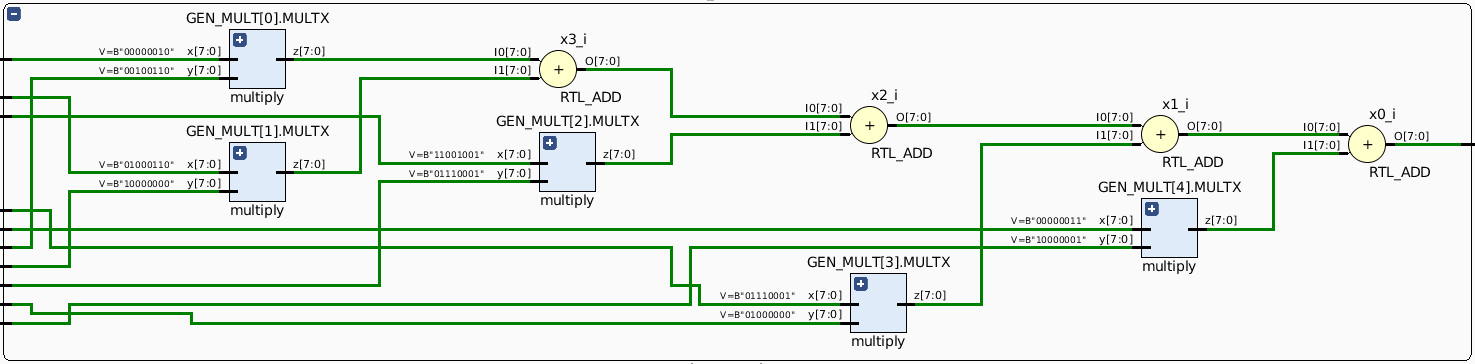
\includegraphics[width=\textwidth]{innerproduct.png}
\caption{A naive implementation of an inner product}
\label{fig:naive_inner_product}
\centering
\end{figure}

The naive construction would produce an output in one clock cycle, giving an extremely good latency.  However it is only feasible for relatively small matrices.  In the neural net architecture chosen for MAIA, matrix multiplication represents about half of the trainable parameters, about $150,000$ coefficients.  The naive implementation would require one DSP slice per parameter, but only 220 DSP slices are available for us to use.  We have not even talked about convolution which makes up the other half of trainable parameters.  It is clear then, that for our large scale problem, we must turn to time domain multiplexing of the hardware.  That is, one matrix multiply must be accomplished over the time frame of many clock cycles, with each DSP slice performing multiple different multiplications.







